
%(BEGIN_QUESTION)
% Copyright 2012, Tony R. Kuphaldt, released under the Creative Commons Attribution License (v 1.0)
% This means you may do almost anything with this work of mine, so long as you give me proper credit

Qualitatively graph the response of an integral-only controller over time to the following changes in process variable:

$$\includegraphics[width=15.5cm]{i01594x01.eps}$$

Assume {\it reverse} control action.

\vskip 20pt \vbox{\hrule \hbox{\strut \vrule{} {\bf Suggestions for Socratic discussion} \vrule} \hrule}

\begin{itemize}
\item{} How would the controller's response differ if it were configured for {\it direct} action instead?
\item{} What factor(s) dictate the use of direct versus reverse controller action?
\item{} Explain why it would be highly unusual to see a trend like this in a real, working process loop.  Why is this trend unrealistic, assuming a working process where all components are functioning properly?
\item{} Given that this trend is unrealistic, why is it something we're studying?  In other words, what value does a ``toy'' trend like this have for us?
\end{itemize}

\underbar{file i01594}
%(END_QUESTION)





%(BEGIN_ANSWER)

The controller output graph shown here is {\it qualitative} only.  Although drawn to scale (i.e. all changes in the output are properly scaled relative to each other), the scale itself is arbitrary and therefore may not match the scale of your sketch:

$$\includegraphics[width=15.5cm]{i01594x02.eps}$$

%(END_ANSWER)





%(BEGIN_NOTES)

{\bf Proportional control action is where the amount of error tells the output how \underbar{far} to go.}

\vskip 10pt

{\bf Integral control action is where the amount of error tells the output how \underbar{fast} to go.}

\vskip 10pt

{\bf Derivative control action is where \underbar{speed} of the error tells the output how \underbar{far} to go.}

\vskip 10pt


Although this question only asks for a {\it qualitative} sketch, it is important for students to take care and make all their sketches as accurate in proportion as they can.  For example, you can see in my answer that the first ramping period changes by 15\%, while the second ramping period changes by only 5\% because the area integrated under the first error period is {\it three times greater} than the area integrated under the second error period.  Students' qualitative sketches should reveal the same 3:1 ratio.

A common misconception many students make is to make the ramping magnitude equal to the error magnitude.  This is wrong because it completely ignores {\it time} as a variable in integration.













\vfil \eject

\noindent
{\bf Summary Quiz:}

Suppose a student sketches this output trend to explain what a direct-acting, integral-only controller would do in response to the two ``steps'' in process variable:

$$\includegraphics[width=15.5cm]{i01594x03.eps}$$

This is {\it not} what a real integral-only controller would do.  Explain what is wrong with the student's sketch of the output.

%INDEX% Control, integral: graphing controller response

%(END_NOTES)


